\documentclass[conference]{IEEEtran}
\IEEEoverridecommandlockouts
% The preceding line is only needed to identify funding in the first footnote. If that is unneeded, please comment it out.
%Template version as of 6/27/2024

\usepackage{cite}
\usepackage{amsmath,amssymb,amsfonts}
\usepackage{algorithmic}
\usepackage{graphicx}
\usepackage{textcomp}
\usepackage{hyperref}
\usepackage{xcolor}
\def\BibTeX{{\rm B\kern-.05em{\sc i\kern-.025em b}\kern-.08em
    T\kern-.1667em\lower.7ex\hbox{E}\kern-.125emX}}
\begin{document}

\title{MOSAIC: A Flexible, Multi-Backend Federated Learning Platform
for Biomedical Research Infrastructure%
\thanks{This work was supported by the National AI Research Resource
(NAIRR) Pilot and the DOE--NIH PALISADE-X project. [Grant numbers to be
added.]}
}

\author{\IEEEauthorblockN{1\textsuperscript{st} Given Name Surname}
\IEEEauthorblockA{\textit{dept. name of organization (of Aff.)} \\
\textit{name of organization (of Aff.)}\\
City, Country \\
email address or ORCID}
\and
\IEEEauthorblockN{2\textsuperscript{nd} Given Name Surname}
\IEEEauthorblockA{\textit{dept. name of organization (of Aff.)} \\
\textit{name of organization (of Aff.)}\\
City, Country \\
email address or ORCID}
\and
\IEEEauthorblockN{3\textsuperscript{rd} Given Name Surname}
\IEEEauthorblockA{\textit{dept. name of organization (of Aff.)} \\
\textit{name of organization (of Aff.)}\\
City, Country \\
email address or ORCID}
\and
\IEEEauthorblockN{4\textsuperscript{th} Given Name Surname}
\IEEEauthorblockA{\textit{dept. name of organization (of Aff.)} \\
\textit{name of organization (of Aff.)}\\
City, Country \\
email address or ORCID}
\and
\IEEEauthorblockN{5\textsuperscript{th} Given Name Surname}
\IEEEauthorblockA{\textit{dept. name of organization (of Aff.)} \\
\textit{name of organization (of Aff.)}\\
City, Country \\
email address or ORCID}
\and
\IEEEauthorblockN{6\textsuperscript{th} Given Name Surname}
\IEEEauthorblockA{\textit{dept. name of organization (of Aff.)} \\
\textit{name of organization (of Aff.)}\\
City, Country \\
email address or ORCID}
}

\maketitle

\begin{abstract}
Federated learning (FL) enables cross-institutional AI model training
without sharing sensitive data, but practical deployment across
national research infrastructure demands flexibility in identity
management, compute backends, and client communication that no
existing FL platform provides. Through the NAIRR Pilot and the
DOE--NIH PALISADE-X project, we established the APPFL ecosystem at
national scale---benchmarking FL algorithms across multiple DOE
supercomputing facilities and deploying across four NIH Bridge2AI
programs---building a solid foundation of validated infrastructure and
deployment experience. That experience revealed clear architectural
gaps: tight coupling to Globus for identity excluded hospital and
institutional users; an AWS-only server backend blocked NERSC and HPC
deployments; and a single communication mode did not fit
environments with strict network policies. We present MOSAIC, the redesigned platform organized around five
interacting layers: a three-tier role model (Admin, Orchestrator,
Client), a unified Keycloak authentication layer accepting Globus,
institutional LDAP, and any OIDC provider, a pluggable computing
resource layer spanning AWS ECS, NERSC Spin/Kubernetes, DOE HPC via
the American Science Cloud, and user-supplied BYOC, a four-mode
application layer covering Globus Compute-based and gRPC-based FL
alongside Jupyter onboarding environments, and a role-scoped
configuration and result tracking layer. This design directly addresses the heterogeneity of national
biomedical research infrastructure while building on the APPFL
algorithmic core and Bridge2AI deployment experience.
\end{abstract}

\begin{IEEEkeywords}
federated learning, federated learning platform, privacy-preserving
AI, biomedical informatics, heterogeneous computing
\end{IEEEkeywords}

%% -----------------------------------------------------------------
\section{Introduction}
%% -----------------------------------------------------------------

Privacy-preserving federated learning (FL) enables institutions to
collaboratively train AI models without sharing sensitive data, making
it an attractive paradigm for biomedical research. Patient records,
genomic sequences, and medical images are distributed across hospitals,
national laboratories, and academic research centers that are subject
to strict privacy regulations, data use agreements, and institutional
governance requirements that prohibit centralization. FL addresses this
by sending model training code to the data: each site trains locally
on its private dataset and shares only model updates, not raw records.
This ``code travels to data'' principle has been demonstrated at scale
in clinical and epidemiological contexts~\cite{rieke2020future,
dayan2021federated, mcmahan2017}.

The APPFL ecosystem~\cite{ryu2022appfl, li2025advances} has
established a comprehensive, production-quality FL framework for
cross-silo research, supporting more than a dozen synchronous and
asynchronous training algorithms, differential privacy, secure
aggregation, and communication-efficient training. Through two
national programs---the NAIRR Pilot and the DOE--NIH PALISADE-X
project---we deployed APPFL at national scale. NAIRR Pilot resources
across multiple DOE supercomputing facilities enabled systematic
benchmarking of FL algorithms, communication protocols, and
privacy-preserving techniques under realistic distributed conditions.
PALISADE-X applied this infrastructure to four NIH Bridge2AI flagship
programs, covering ophthalmology imaging, voice biomarkers, critical
care, and genomics. Together, these programs validated the APPFL
algorithms, stress-tested the deployment infrastructure, and produced
practical experience with the governance and data readiness challenges
that accompany real cross-institutional FL. The result is a solid
foundation.

That same deployment experience, however, revealed a clear set of
architectural gaps in the original APPFLx service~\cite{li2023appflx}.
\textit{Identity management} is tightly coupled to Globus Auth and
Globus Groups: institutions that use LDAP-based campus identity systems
or hospital-operated OIDC providers cannot participate without adopting
Globus, which is not always permissible in clinical environments with
strict data governance requirements.
\textit{Server compute} is AWS-only: research groups that operate
primarily on NERSC or want to leverage DOE HPC allocations for FL
coordination---a natural fit given NAIRR's multi-facility compute
model---cannot use the platform.
\textit{Communication} relies exclusively on Globus Compute function
dispatch, which requires outbound connectivity to the Globus cloud;
hospital networks and secured clinical environments that restrict
external cloud traffic cannot use this path.
\textit{Role management} is informal: the original system has no
structured notion of who can create federations, what data each
participant can see, or how compute resources should be governed as
the platform scales beyond a single research group.

This paper presents MOSAIC (Multi-backend Orchestration Service for
federated AI Collaboration), which addresses all four gaps while
preserving full compatibility with the existing APPFL algorithmic
layer and the Globus-centric users it currently serves. The platform is organized around five interacting layers:

\begin{itemize}
  \item \textbf{Roles:} A three-tier model (Admin, Orchestrator,
  Client) with federation-scoped visibility and lightweight resource
  governance appropriate for a trusted, multi-group research platform.

  \item \textbf{Authentication:} A unified Keycloak layer accepting
  Globus, institutional LDAP/AD, and any OIDC-compliant provider,
  normalizing all users into a single model and issuing standard JWTs
  for stateless validation across API and gRPC services.

  \item \textbf{Computing Resources:} Pluggable server backends---AWS
  ECS, NERSC Spin/Kubernetes, DOE HPC via the American Science Cloud
  (AmSC), and user-supplied Bring Your Own Compute (BYOC)---each
  implementing the same provisioning interface so the choice is
  transparent to upper layers.

  \item \textbf{Applications:} Four application types covering
  Globus Compute-based FL, gRPC-based FL, and Jupyter onboarding
  environments for each communication mode.

  \item \textbf{Configuration \& Result Tracking:} Persistent,
  versioned experiment configuration, live metric streaming via
  WebSocket, and role-scoped result visibility that gives Clients the
  same view of global training metrics as the Orchestrator.
\end{itemize}

Application~1 (Globus Compute FL Orchestrator) is the currently
deployed path and is validated through NAIRR and Bridge2AI experiments.
Applications~2--4 and the Keycloak/Spin backend extensions represent
the next development phase, completing the platform's coverage of the
infrastructure heterogeneity encountered in national biomedical
research.

%% -----------------------------------------------------------------
\section{Background and Related Work}
%% -----------------------------------------------------------------

\subsection{APPFL: The Federated Learning Framework}

APPFL~\cite{ryu2022appfl, li2025advances} is an open-source, modular
FL framework built for cross-silo research on heterogeneous
infrastructure. It supports a broad set of synchronous aggregation
strategies---FedAvg, FedProx, FedAdam---alongside asynchronous
strategies designed for heterogeneous client environments where
stragglers would otherwise bottleneck synchronous rounds: FedBuff
accumulates updates asynchronously while the server continues training,
and FedCompass~\cite{li2024fedcompass} uses a computing power-aware
scheduler that prioritizes faster clients to achieve near-linear
wall-clock scaling. Privacy is enforced via local and global
differential privacy~\cite{dwork2014} and secure
aggregation~\cite{bonawitz2017}. Communication compression---top-$k$
gradient sparsification and quantization---reduces bandwidth cost for
WAN-connected institutional FL. A fully modular architecture allows
plug-in of custom aggregation strategies, privacy mechanisms, and
dataloaders without modifying the core framework, enabling
reproducible benchmarking of individual design choices.

Beyond the core framework, APPFL-related work includes ABLE (Argonne's
Biomedical Learning Environment), a secure computing enclave combining
containerized execution, institutional identity integration (InCommon,
NIH eRA Commons), and encrypted communication channels to support FL
workflows on controlled-access biomedical datasets satisfying HIPAA and
data use agreement requirements. FedSpaLLM~\cite{bai2025fedspalllm}
extends APPFL to the large language model setting via structured
pruning, enabling communication-efficient federated fine-tuning of
LLMs. Together, these components form a growing ecosystem built on a
common, open-source FL core.

\subsection{Original APPFLx}

APPFLx~\cite{li2023appflx, hoang2025appflx} provides FL-as-a-service
on top of APPFL. Its architecture has four layers: (1)~Globus Auth and
Globus Groups for identity management and federation membership---a
``federation'' is a Globus Group, and inviting a client adds them to
that group; (2)~a Flask/React web dashboard where the Orchestrator
configures experiments and Clients register their Globus Compute
endpoint UUIDs and upload dataloaders; (3)~Globus Compute for training
dispatch---the server submits a \texttt{local\_train} Python function
call to each client endpoint each round, Globus cloud relays the call,
and the client's local compute executes it; and (4)~AWS S3 for model
weight staging between the server and clients. The server itself runs
as an AWS ECS Fargate container managed by the platform's AWS account.

This design has proven effective: it handles the asynchronous function
dispatch pattern naturally, requires no inbound ports on client
machines, and the Globus-relayed communication penetrates most HPC
firewalls. However, it constrains every participating institution to
Globus identity, every FL coordinator to AWS compute, and every client
communication path to the Globus cloud relay---constraints that the
Bridge2AI and NAIRR experience revealed as practically significant
exclusion criteria.

\subsection{Related FL Platforms}

NVIDIA FLARE~\cite{roth2022} provides production FL infrastructure
with a focus on medical imaging, supporting diverse aggregation
strategies and privacy mechanisms within a controller--executor
architecture. Flower~\cite{beutel2020flower} is a general-purpose,
framework-agnostic FL research system with flexible server--client
communication and support for many ML backends. Both are strong
algorithm-layer platforms but do not address multi-backend server
provisioning across heterogeneous HPC and cloud infrastructure, or the
multi-identity-provider authentication challenge that arises when
participating institutions span hospitals, national laboratories, and
academic centers with different identity governance models. MOSAIC
occupies a complementary design point: FL-as-a-service with
pluggable compute backends and a unified authentication layer, built on
the APPFL algorithmic core validated at national scale.

%% -----------------------------------------------------------------
\section{MOSAIC Platform Design}
%% -----------------------------------------------------------------

Fig.~\ref{fig:architecture} illustrates how the five layers interact
through the web portal. Users authenticate via the portal, which
validates all requests through the Keycloak auth layer. Orchestrators
configure and launch experiments through the portal; the platform
deploys the selected application to the chosen compute backend and
streams results from the tracking layer back to all authorized users
in real time.

\begin{figure}[t]
  \centering
  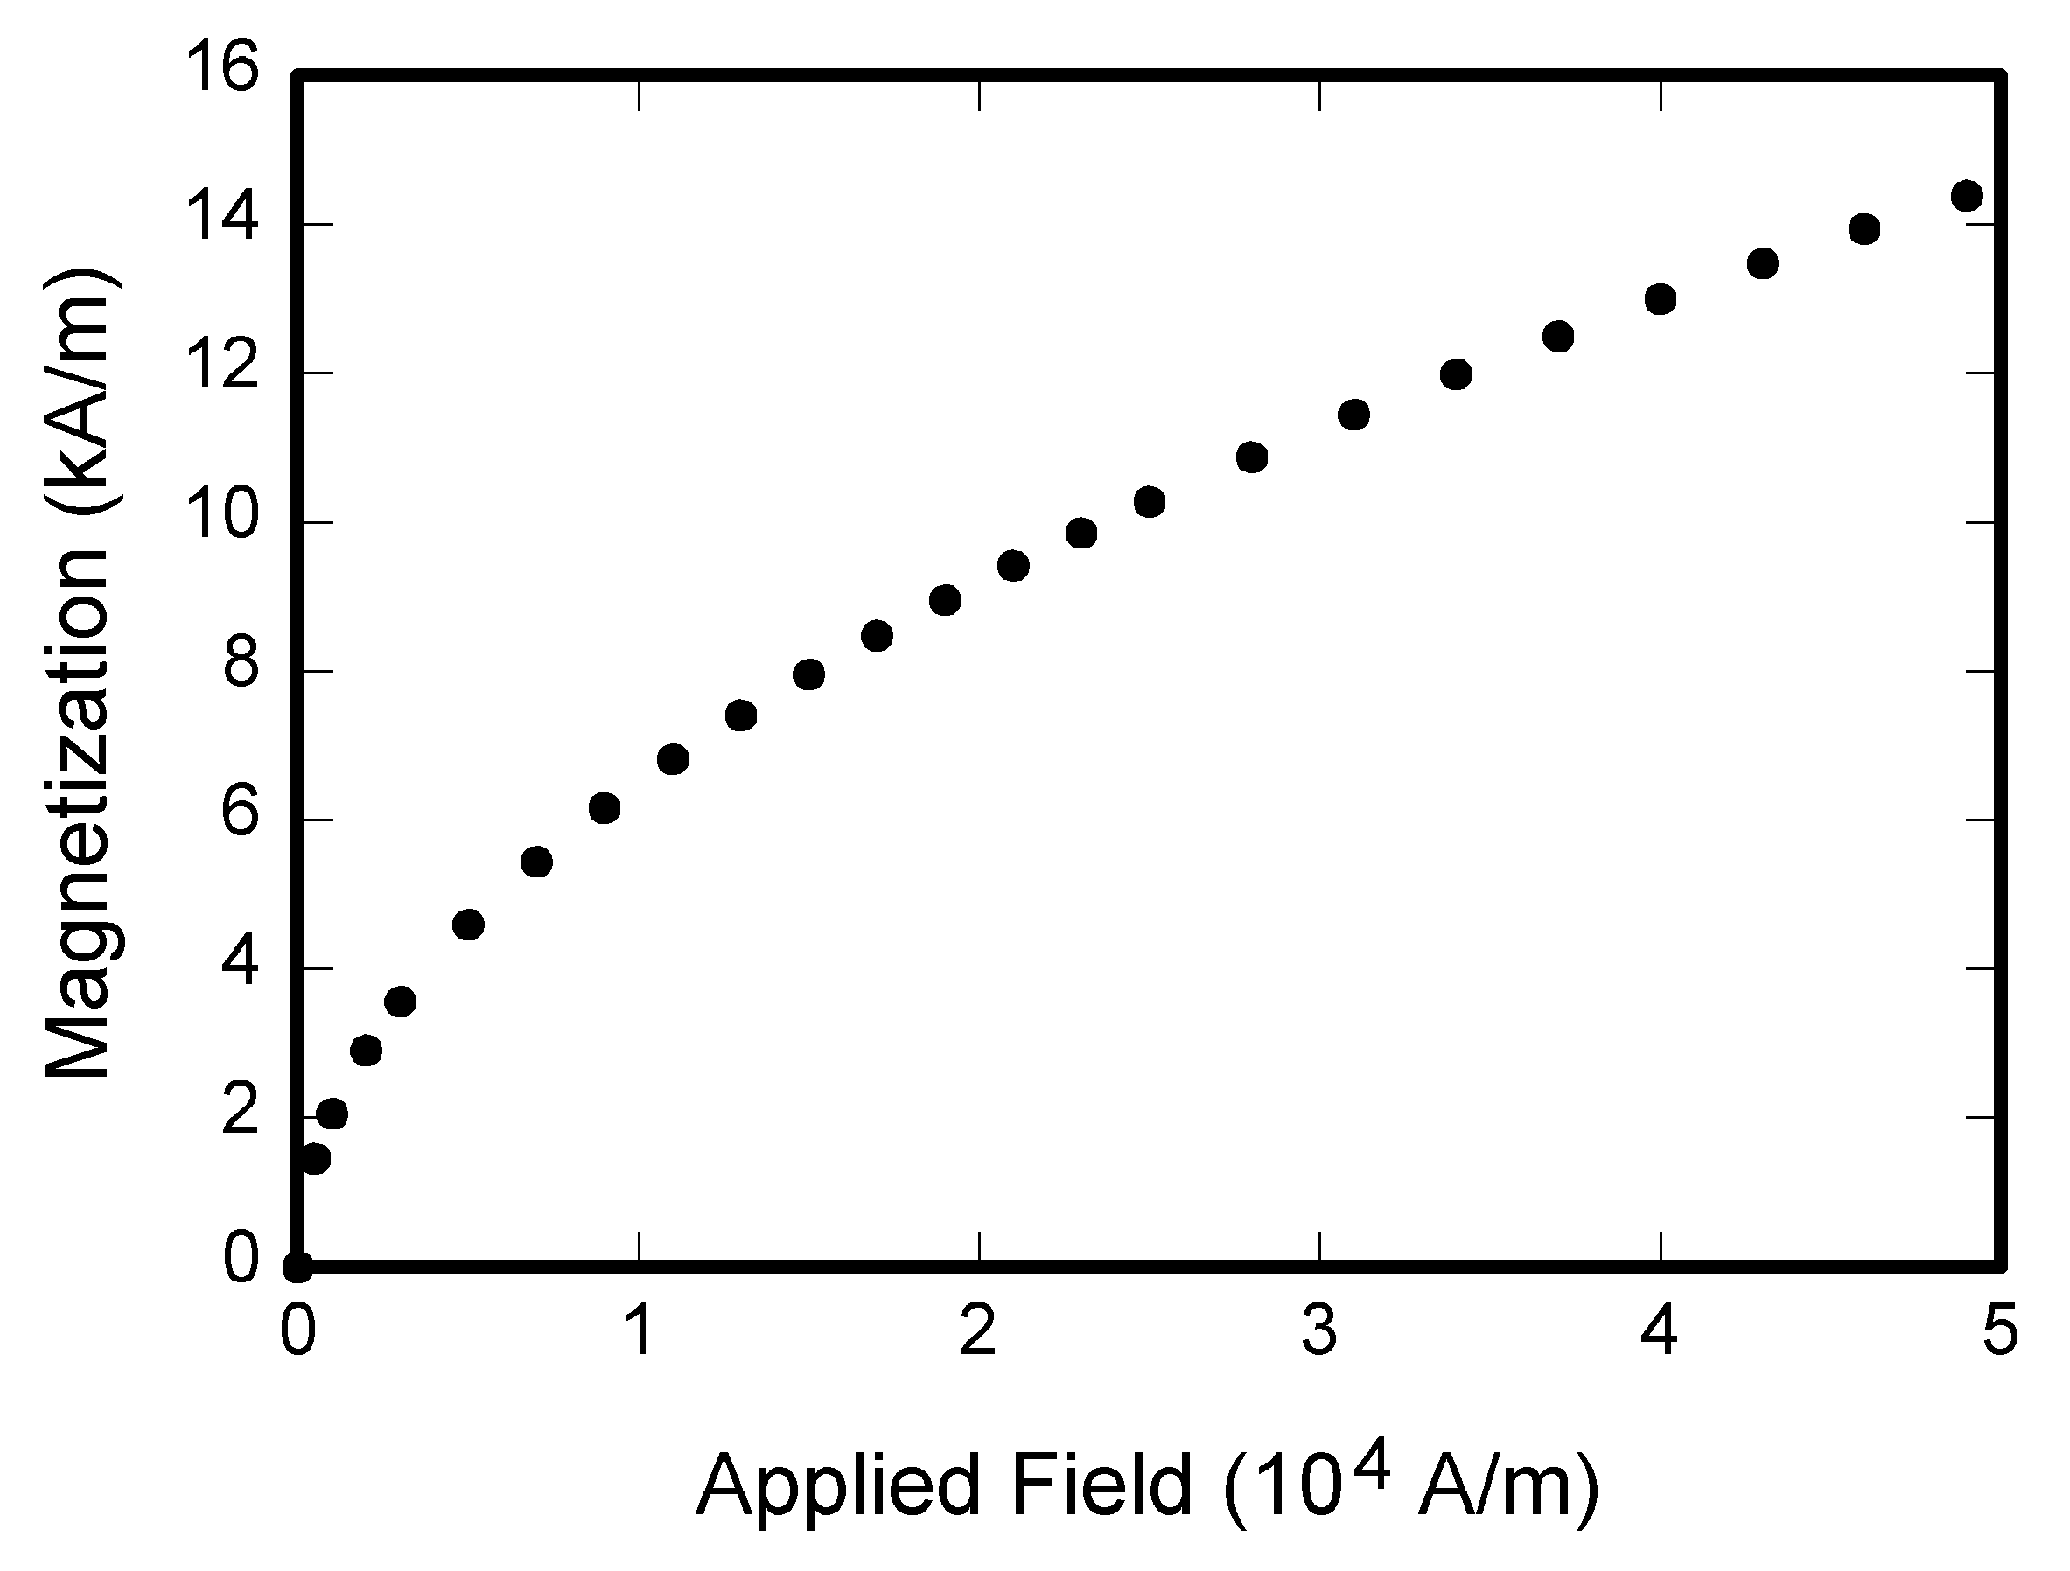
\includegraphics[width=\columnwidth]{fig1.png}
  \caption{MOSAIC platform architecture. The web portal is the central
  interaction point for all three roles. The Keycloak authentication
  layer validates every request. The portal deploys applications to the
  selected compute backend and streams per-round training metrics back
  to Orchestrators and Clients via WebSocket. Clients interact with
  deployed FL applications directly at runtime via Globus Compute calls
  or gRPC connections.}
  \label{fig:architecture}
\end{figure}

\subsection{Role-Based Access Control}

Three roles operate in a strict hierarchy: Admin $\to$ Orchestrator
$\to$ Client. Role assignment is managed through the Keycloak admin
interface and reflected in every JWT issued by the platform.

\textbf{Admin} is the platform operator (in the current context, the
research group running the platform). The first Admin account is
bootstrapped at platform setup; subsequent Admin grants are made
through the Keycloak console or the platform portal. Admins approve and
elevate registered users to Orchestrator status---self-registration
does not automatically grant federation-creation privileges. Admins
configure available compute backends, set per-Orchestrator resource
limits (maximum concurrent experiments, maximum wall-clock experiment
duration with automatic teardown), and monitor platform-wide usage.
Critically, Admins see only non-sensitive aggregate operational
metadata: which federations exist, member counts, experiment counts,
backend types, and compute time consumed. They do not see model
architectures, training datasets, hyperparameters, training metrics,
or any content-level experiment information.

\textbf{Orchestrator} is a researcher authorized to create and manage
federations. Orchestrators create federations (choosing a compute
backend per experiment, not per federation), invite Clients by email
or platform identity, configure FL experiments (model architecture,
training algorithm, differential privacy budget, number of rounds,
evaluation metrics), trigger AIDRIN data readiness inspections, launch
experiments, and access the full set of experiment results including
per-round global model metrics, per-client participation logs, and the
final trained model. Resource limits apply only to experiments using
MOSAIC-provided compute (ECS, Spin, AmSC); BYOC experiments are not
subject to platform resource constraints. A single federation can host
experiments of multiple application types across its lifetime.

\textbf{Client} is a data-holding institution invited into a
federation by an Orchestrator. The invitation flow begins when the
Orchestrator sends an invite through the portal; the invitee follows
a link, authenticates via Keycloak using any supported identity
provider, accepts the invitation, and appears in the federation. No
Admin approval is required---the Orchestrator controls federation
membership entirely. Clients provide local compute resources at their
own site; the platform provisions nothing on their behalf. Raw data
never leaves the Client's site---only locally computed model updates
are transmitted. Clients access the same set of FL experiment results
as the Orchestrator: per-round global model performance metrics,
per-client participation status, aggregated AIDRIN readiness reports,
server-side logs, and the final model. They additionally see their own
per-round local training metrics. They do not see other clients' local
metrics.

\subsection{Authentication Layer}

All identity and access management flows through a self-hosted
Keycloak instance, deployed as a containerized service on the same
infrastructure as the rest of the platform. Keycloak is an
open-source identity and access management server supporting standard
OAuth2/OIDC flows and LDAP integration.

Keycloak normalizes multiple identity sources into a single platform
user model. Globus is registered as a federated external OIDC identity
provider within Keycloak: a user who authenticates via Globus is
transparently mapped to a Keycloak user record, and the platform API
receives a Keycloak-issued JWT regardless of which underlying identity
provider was used. Institutional LDAP and Active Directory directories
can be connected directly, enabling users to log in with their existing
organizational credentials. Any OIDC-compliant external identity server
can similarly be registered as a provider. The result is that the
platform is not locked to any single identity ecosystem: a Globus user
and a hospital LDAP user participating in the same federation are
treated identically at the API level.

Platform-level roles (Admin, Orchestrator) are encoded as Keycloak
realm roles and appear as claims in the issued JWT. Federation
membership is implemented as Keycloak Groups: creating a federation
creates a corresponding group; accepting a Client invitation adds the
user to that group with a Client-scoped role. Every API endpoint and
gRPC service validates incoming JWTs against Keycloak's public JWKS
endpoint---stateless validation with no runtime callback to the portal,
enabling high-throughput gRPC servers and intermittently-connected
deployments.

For gRPC-mode experiments, the platform generates a
federation-scoped JWT (signed by Keycloak) and makes it available for
download by each Client through the portal. The Client's training
script presents this token to the gRPC server, which validates it
independently. This token-download flow means gRPC clients do not need
an active connection to the portal during training.

\subsection{Computing Resource Layer}

The compute layer implements a uniform interface: deploy a container
image with a given configuration, expose a network endpoint, stream
logs to the platform, and tear down the container when the experiment
ends or a maximum-duration timeout is reached. All backends implement
this interface; the Orchestrator selects a backend per experiment, and
upper layers are unaware of the underlying infrastructure.

\textbf{AWS ECS} is the currently deployed backend. The platform
launches the FL server as a Fargate task inside its own AWS account,
using IAM roles scoped per federation for isolation. AWS S3 stores
model weight checkpoints and CloudWatch collects server logs. No NERSC
account is required from the user.

\textbf{NERSC Spin} is NERSC's containers-as-a-service platform, built
on Rancher-managed Kubernetes. The platform deploys via the Kubernetes
API: a \textit{Deployment} object keeps the server container running
and restarts it on failure; a \textit{Service} object provides a
stable internal DNS name; and an \textit{Ingress} object exposes a
public TLS-terminated endpoint using automatic certificate management.
Spin containers can mount NERSC Collaborative File System and scratch
storage directly as persistent volumes, eliminating the need to stage
model weights to an external object store for NERSC-based experiments.
Spin incurs no per-experiment cloud cost, making it well-suited for
research groups with established NERSC allocations.

\textbf{AmSC / DOE HPC} uses the American Science Cloud
SDK~\cite{amsc} to submit the FL coordinator as a batch job on DOE
HPC systems---currently ALCF (Polaris, Aurora, Sophia via PBS) and
NERSC (Perlmutter via Slurm)---through a unified Facility API that
abstracts over site-specific job schedulers. This backend provides
access to leadership-class GPU allocations for computationally
intensive coordination tasks such as server-side aggregation of large
model updates. AmSC integrates Globus authentication, which reuses the
Globus IdP already registered within the platform's Keycloak instance
with no additional login step. A key constraint: HPC compute nodes
do not accept inbound network connections from outside the facility,
so the AmSC backend is compatible only with Globus Compute-mode
experiments, where the server requires only outbound connectivity to
the Globus cloud to dispatch function calls to client endpoints.
AmSC also provides a Catalog API for discovering DOE-hosted scientific
datasets and a Filesystem API for staging model artifacts across ALCF
and NERSC storage systems.

\textbf{BYOC} allows Orchestrators to supply their own compute
credentials---an AWS cross-account IAM role ARN for ECS deployments or
a namespace credential for their own NERSC Spin allocation. The
platform deploys into their infrastructure using the same mechanisms as
the platform-managed backends; no platform compute budget is consumed
and no platform resource limits are imposed. BYOC is the recommended
path for Orchestrators running regular large-scale experiments.

\subsection{Application Layer}

An \emph{application} pairs a server-side container image with a
corresponding client interaction pattern. Table~\ref{tab:apps}
summarizes the four application types. The application type is selected
per experiment rather than per federation, so a single federation can
host experiments of different types as its participants or requirements
evolve.

\begin{table}[t]
\caption{MOSAIC Application Types}
\label{tab:apps}
\begin{center}
\renewcommand{\arraystretch}{1.15}
\begin{tabular}{p{1.5cm} p{1.6cm} p{2.0cm} p{1.6cm}}
\toprule
\textbf{Application} & \textbf{Compatible Backends$^{\dagger}$} & \textbf{Client Setup} & \textbf{FL Mode} \\
\midrule
App~1: GC Orch.$^{*}$
  & All
  & GC endpoint + dataloader
  & Sync \& Async \\
App~2: gRPC Server
  & ECS, Spin, K8s, BYOC
  & Download template script
  & Sync \& Async \\
App~3: Jupyter (GC)
  & ECS, Spin, BYOC
  & Start GC endpoint, share UUID
  & Interactive \\
App~4: Jupyter (gRPC)
  & ECS, Spin, BYOC
  & Run local notebook
  & Interactive \\
\bottomrule
\multicolumn{4}{l}{\small $^{*}$Currently deployed. $^{\dagger}$Server-side backend only.}
\end{tabular}
\end{center}
\end{table}

\textbf{Application 1: Globus Compute FL Orchestrator.} This is the
currently supported and deployed application, validated through NAIRR
and Bridge2AI experiments. The server acts as a coordinator: each FL
round dispatches a \texttt{local\_train} Python function call to each
Client's registered Globus Compute endpoint via the Globus cloud relay.
The Globus cloud relays these calls without requiring the client to
open any inbound firewall ports---clients need only outbound access to
Globus, making this suitable for HPC clients behind institutional
network policies. Clients register a Globus Compute endpoint UUID
through the platform portal and upload a \texttt{dataloader.py} file
describing their local dataset loading logic. The FaaS dispatch model
makes this application naturally suited to asynchronous FL algorithms
(FedCompass, FedBuff), where the server can issue function calls to
available clients without waiting for the full cohort, and compatible
with all server backends including AmSC/HPC.

\textbf{Application 2: gRPC FL Server.} The server runs a persistent
gRPC service with a publicly accessible endpoint, exposed via a
Kubernetes Ingress (with automatic TLS certificate management) or an
ECS load balancer. A key design point: in APPFL's gRPC implementation,
the \emph{client} controls the training loop rather than the server.
Clients decide when to pull the current global model from the server,
when to push locally computed updates, and what types of requests to
issue---the server is reactive. This client-controlled loop supports
both synchronous and asynchronous FL strategies. Clients download a
customizable template training script from the portal, containing the
gRPC server URI and a Keycloak-issued JWT scoped to their federation.
The template exposes configuration options for each client's local
setup: whether to run AIDRIN data readiness checks before training
begins, local training hyperparameters, and dataloader configuration.
gRPC operates over HTTP/2 on port 443, making it compatible with most
enterprise firewall policies---including clinical and hospital
environments where Globus cloud connectivity is unavailable. The gRPC
backend is not compatible with AmSC/HPC due to the inbound connection
constraint of HPC compute nodes.

\textbf{Application 3: Jupyter Server -- Globus Compute Notebooks.}
This application provides a zero-setup onboarding environment for the
Globus Compute FL workflow. The platform deploys a containerized
Jupyter server with all required packages pre-installed (\texttt{appfl},
\texttt{globus-compute-endpoint}, and their dependencies). The
Orchestrator accesses the server via a direct link and a one-time
access token provided by the platform portal after deployment---no
Keycloak SSO is used to access the Jupyter interface itself. Pre-loaded
notebooks walk through registering a Globus Compute endpoint, writing
and testing a dataloader for a sample dataset, configuring and
launching a small-scale FL experiment via the APPFL Python API, and
interpreting training metrics. Clients do not connect to the Jupyter
server; they only need to start their own Globus Compute endpoints on
their local compute resources and provide the endpoint UUID to the
Orchestrator, who enters it into the notebook configuration cells.
Once participants are confident in their setup, they transition to
Application~1 for production-scale experiments.

\textbf{Application 4: Jupyter Server -- gRPC Notebooks.} An
analogous onboarding environment for the gRPC FL path. The platform
deploys a Jupyter server (accessed by the Orchestrator via link and
token) containing notebooks that walk through configuring a gRPC FL
server and monitoring per-round metrics from the orchestrator's
perspective. For Clients, the onboarding model is different from
Application~3: rather than accessing a shared online server, each
Client downloads a pre-configured \texttt{.ipynb} notebook file from
the platform portal and runs it in their own local Jupyter environment.
The notebook guides them through connecting to the gRPC server,
validating their local dataloader, and running the client-side training
loop interactively, providing a low-friction entry point that requires
only a standard Python environment with \texttt{appfl} installed.

\subsection{Configuration and Result Tracking}

Experiment configuration is collected through the portal at launch
time and stored in a persistent database versioned per experiment,
enabling reproducibility. Common parameters---model architecture,
training algorithm, differential privacy settings, number of rounds,
evaluation metric---are specified by the Orchestrator. Application-
specific parameters are collected per role: for Globus Compute
experiments, each Client's endpoint UUID and dataloader; for gRPC
experiments, the server URI and Client JWT are auto-generated and
surfaced for Client download.

During training, the FL server reports per-round results to the
platform API at the end of each round. The portal streams these
results live to Orchestrators and Clients alike via WebSocket: global
model performance metrics (loss, accuracy, AUC, or other configured
metric) plotted as a curve, and per-client participation status per
round (contributed / timed out / skipped). After completion, model
artifacts---checkpoints, the final global model, and AIDRIN readiness
reports---are stored in S3 for ECS-backed experiments or on NERSC
filesystems for Spin-backed experiments, and retained for a
configurable period before deletion, with experiment metadata kept
indefinitely for Admin audit.

\textbf{AIDRIN integration.} AIDRIN~\cite{hiniduma2024aidrin,
hiniduma2025aidrin2} can be triggered by the Orchestrator before an
experiment launches. Each Client runs AIDRIN locally against their
private dataset, evaluating completeness (missing values, label
coverage), harmonization readiness (OMOP/FHIR alignment), cohort
representation (demographic distributions computed with differential
privacy before upload), and AI-suitability for the configured model.
Each Client submits a privacy-preserving summary---not raw data---to
the platform API. The platform aggregates these summaries and presents
the Orchestrator with a readiness dashboard: which sites are ready,
which have issues, and AIDRIN's recommended remediation steps. The
Orchestrator decides whether to proceed or ask specific clients to
address issues first. CADRE~\cite{hiniduma2025cadre} extends this
evaluation into the FL training loop itself, checking data readiness
at the start of each round to detect drift or site-level quality
degradation mid-experiment without exposing raw data.

%% -----------------------------------------------------------------
\section{Foundation: NAIRR Pilot and Bridge2AI Experience}
%% -----------------------------------------------------------------

The redesigned MOSAIC platform is not built from scratch---every
design decision is grounded in two national programs that provided
both the infrastructure resources and the concrete, sometimes
uncomfortable, deployment experience that revealed what a production
FL platform for national biomedical research actually needs.

\subsection{NAIRR Pilot: Benchmarking FL at Scale}

The NAIRR Pilot allocation provided access to ALCF and NERSC
supercomputing facilities, enabling FL experiments under realistic
distributed conditions at scales unavailable to individual institutions.
We systematically benchmarked synchronous and asynchronous FL
strategies, gradient compression techniques, and differential privacy
mechanisms across geographically separated compute sites.

\textbf{Algorithm scalability.}
Table~\ref{tab:algorithms} compares FL strategies across increasing
numbers of simulated clients. Asynchronous algorithms (FedBuff,
FedCompass~\cite{li2024fedcompass}) substantially reduce wall-clock
time in heterogeneous client environments, where a single slow client
would otherwise bottleneck all synchronous rounds. FedCompass's
computing power-aware scheduler dynamically assigns workloads
proportional to each client's available compute, achieving near-linear
wall-clock scaling in heterogeneous settings at modest accuracy cost.

\begin{table}[t]
\caption{FL Algorithm Comparison on NAIRR Resources}
\label{tab:algorithms}
\begin{center}
\begin{tabular}{l c c c}
\toprule
\textbf{Algorithm} & \textbf{Type} & \textbf{Accuracy} & \textbf{Wall-clock} \\
\midrule
FedAvg      & Sync  & [XX]\% & [X.X] h \\
FedProx     & Sync  & [XX]\% & [X.X] h \\
FedAdam     & Sync  & [XX]\% & [X.X] h \\
FedBuff     & Async & [XX]\% & [X.X] h \\
FedCompass  & Async & [XX]\% & [X.X] h \\
\bottomrule
\multicolumn{4}{l}{\small [Benchmark numbers to be filled from NAIRR experiments.]}
\end{tabular}
\end{center}
\end{table}

\textbf{Communication efficiency.}
Communication cost dominates training time in geographically
distributed FL. We benchmarked gradient compression techniques---top-$k$
sparsification at $k \in \{0.1\%, 1\%, 10\%\}$ and quantization at
\{4, 8, 16\} bits---against uncompressed baselines across biomedical
imaging and clinical text tasks. Top-$k$ sparsification at 10\%
reduces communication volume by $10\times$ with less than 0.5\%
accuracy degradation, a practically important trade-off for
WAN-connected institutional clients. These results informed the
multi-protocol design of the application layer: gRPC's binary HTTP/2
framing is significantly more bandwidth-efficient than REST-based
alternatives for dense model parameter exchange, particularly relevant
for large model architectures. FedCostAware~\cite{sinha2025fedcostaware}
extends communication efficiency with cloud-cost-aware scheduling,
dynamically selecting cost-efficient resource configurations to reduce
total training cost, directly informing the BYOC design.

\textbf{Privacy-utility trade-off.}
Using NAIRR resources, we characterized the differential privacy
trade-off across $\varepsilon \in \{1, 2, 5, 10, \infty\}$ for
medical imaging and clinical text tasks. Differential privacy at
$\varepsilon = 5$--$10$ provides meaningful privacy guarantees with
less than 2\% accuracy degradation---a practically actionable
guideline for IRB negotiations about acceptable privacy budgets in
federated clinical AI studies. The NAIRR experiments confirmed that
the APPFL privacy mechanisms work correctly at multi-site scale and
that the privacy budget trades off gracefully across a range of
task types.

These NAIRR experiments validated the APPFL algorithmic core and
directly shaped the MOSAIC backend design. The practical need to run
FL coordinators on DOE HPC allocations---where leadership-class GPU
capacity dwarfs what either ECS or Spin can provide for aggregation
of large model updates---motivated the AmSC backend. The prevalence
of Globus-authenticated HPC users motivated preserving Globus as a
first-class identity provider within Keycloak rather than replacing it.

\subsection{PALISADE-X and Bridge2AI Deployments}

PALISADE-X deployed APPFL across four NIH Bridge2AI flagship programs.
Each program posed distinct infrastructure, governance, and data
challenges that directly motivated specific design choices in the
redesigned MOSAIC.

\textbf{AI-READI}~\cite{aireadi_arvo} is building AI-ready datasets
for retinal disease research---including geographic atrophy and
age-related macular degeneration---across multiple academic medical
centers. Using APPFL, we developed and validated federated workflows
for training retinal image classifiers while imaging and clinical data
remain at each participating institution. Federated models achieved
accuracy comparable to centralized baselines while improving
generalizability across the demographic heterogeneity of participating
cohorts, consistent with the expected benefit of training on a broader
and more representative distributed dataset. Workshops and tutorials
at the Association for Research in Vision and Ophthalmology (ARVO)
conference reached several hundred ophthalmologists and biomedical AI
researchers, establishing reusable workflow templates. The AI-READI
deployments confirmed that the Globus Compute path works well for
academic medical center clients with established research computing
infrastructure.

\textbf{Voice AI}~\cite{b2ai_voice_fl} investigates FL for training
speech biomarker detection models that can identify neurological,
respiratory, behavioral, and cognitive conditions from voice recordings.
Voice data is among the most personally identifying data types, making
centralization especially problematic for consent and re-identification
risk. These experiments produced practical insights into the specific
challenges of federated training with large audio datasets---a modality
underrepresented in the FL literature---including high communication
costs for large audio model weights and the need for differential
privacy mechanisms adapted for high-dimensional audio gradient spaces.
Critically, hospitals contributing voice datasets often operate networks
that block outbound connectivity to Globus cloud, directly motivating
the gRPC application path as an alternative communication mode.

\textbf{CHoRUS} targets early prediction of sepsis onset from
multimodal clinical datasets across critical care units at multiple
academic medical centers. The most instructive finding from CHoRUS
engagement was that non-technical prerequisites consumed as much effort
as the technical FL implementation: negotiating data use agreements
with collaborating institutions, harmonizing IRB protocols across sites,
and implementing audit logging sufficient to satisfy institutional data
governance requirements each required substantial time that was not
originally anticipated. This experience directly motivated the AIDRIN
and CADRE integration in MOSAIC: both data quality and governance
readiness must be assessed and validated at each site before FL
experiments begin, not discovered after model training has started and
results are already contaminated by a site's data quality issue.

\textbf{Genomics / GA4GH.} Large-scale biobanks generating genomic
datasets valuable for AI research frequently cannot be centralized due
to privacy regulations, institutional policies, and international
governance requirements that vary across jurisdictions. PALISADE-X
integrated APPFL with GA4GH Task Execution Service (TES) for portable
task submission and Data Repository Service (DRS) for standardized
dataset discovery and access~\cite{ga4gh}. These integrations allow
APPFL-orchestrated FL workflows to operate within emerging
international genomics infrastructure without deploying APPFL-specific
client software at each repository. PALISADE-X proposed and now leads
a GA4GH Federated Learning working group developing open standards and
best practices for FL experiment orchestration across distributed
genomics repositories and biobanks internationally. The diversity of
identity systems encountered across genomics institutions---some using
Globus, others using institutional OIDC or LDAP systems---was among
the most concrete motivations for replacing the Globus-only auth model
with Keycloak's multi-provider approach.

%% -----------------------------------------------------------------
\section{Discussion}
%% -----------------------------------------------------------------

\subsection{Current State and Roadmap}

Application~1 (Globus Compute FL Orchestrator) with the AWS ECS
backend is currently deployed and production-validated. The highest
priority next steps are: (1) deploying the Keycloak authentication
layer, which unblocks all institutions that cannot use Globus for
identity management; (2) adding the NERSC Spin backend, which gives
NERSC-resident research groups an alternative to AWS without requiring
cloud budgets; and (3) implementing Application~2 (gRPC FL Server),
which opens the platform to hospital networks and other environments
where Globus Compute is unavailable. The Jupyter onboarding
applications (3 and 4) are lower priority but high-value for
community adoption, as they lower the barrier for new participants to
validate their setup before committing to a production experiment.

\subsection{Design Trade-offs and Lessons Learned}

The original APPFLx achieved operational simplicity by fixing the
identity provider, compute backend, and communication mode. Every
participant had to meet the platform on its terms. The redesigned
platform inverts this: the platform meets participants where they are
by making each dimension independently pluggable. The cost is
implementation complexity in the platform layer---but that complexity
is paid once by the platform team rather than repeatedly by each
research group trying to adapt a single-mode system to their
environment.

A second important trade-off is between resource governance strictness
and usability. For a small, trusted user base, heavy quota enforcement
creates friction without proportionate benefit. The current design
applies lightweight controls only to MOSAIC-provided compute
(automatic experiment teardown at the maximum duration limit; a cap on
concurrent experiments per Orchestrator) and imposes no limits on BYOC
experiments. This is deliberately permissive for a research platform;
if the user base grows significantly or the platform opens to external
users, BYOC becomes the recommended path that removes cost burden from
the platform entirely.

The AmSC/HPC backend introduces one hard architectural constraint: HPC
compute nodes do not accept inbound connections, making gRPC-mode
experiments incompatible with this backend. This is a constraint of
the HPC environment's network architecture, not a design flaw, and it
is surfaced explicitly in the application--backend decision matrix
(Table~\ref{tab:apps}) so Orchestrators understand it upfront.

\subsection{Future Work}

Several open technical problems remain. First, the Keycloak + Globus
OIDC federation requires careful token handling: when a user
authenticates through Keycloak via Globus, obtaining Globus Compute
credentials (which are separate from the OIDC identity token) for
dispatching function calls to Globus Compute endpoints is not
straightforward and requires a token exchange flow that has not yet
been fully specified. This is the most technically uncertain part of
the authentication design. Second, large model weight transfer in
gRPC mode---for LLMs or large vision models whose parameter vectors do
not fit within a single gRPC message---requires an out-of-band staging
module (S3 pre-signed URLs or Globus Transfer) that can be swapped per
backend without changing the gRPC protocol layer. Third, as the
platform scales to more federations and participants, the federation
lifecycle management (experiment teardown, artifact retention, member
removal) needs to be more automated. Fourth, integrating machine-readable
data governance---encoding data use conditions using ODRL or the GA4GH
Data Use Ontology (DUO)---would allow the platform to verify
experiment--dataset compatibility automatically at the AIDRIN stage,
rather than relying on manual Orchestrator review.

%% -----------------------------------------------------------------
\section{Conclusion}
%% -----------------------------------------------------------------

The NAIRR Pilot and PALISADE-X programs established APPFL as
production-quality FL infrastructure for national biomedical research,
validating its algorithmic core at multi-facility scale and deploying
it across four NIH Bridge2AI programs covering the major data modalities
of biomedical AI. That foundation also revealed a clear gap: a
single-backend, single-protocol, Globus-only FL service cannot serve
the full heterogeneity of institutions, compute environments, and
network configurations that national biomedical research requires.

The redesigned MOSAIC addresses this through five independently
pluggable layers: a three-tier role model with formal federation
governance, a Keycloak-unified authentication layer that accepts
Globus, institutional LDAP, and any OIDC-compliant provider, a
compute resource layer spanning AWS ECS, NERSC Spin/Kubernetes, DOE
HPC via AmSC, and BYOC, a four-mode application layer covering both
production FL communication modes and lightweight Jupyter onboarding
environments, and a role-scoped configuration and result tracking layer
with integrated AIDRIN/CADRE data readiness assessment. Together, these
layers extend the proven APPFL core to the broader range of
participants and infrastructure that national biomedical research
actually uses---without abandoning the Globus ecosystem that the
existing user base depends on.

%% -----------------------------------------------------------------
\section*{Acknowledgment}
%% -----------------------------------------------------------------

This work was supported by the National AI Research Resource (NAIRR)
Pilot [grant numbers to be added] and the DOE--NIH PALISADE-X project
[grant numbers to be added]. The authors acknowledge computing
resources provided by Argonne National Laboratory and the National
Energy Research Scientific Computing Center (NERSC) through the NAIRR
Pilot program. We thank collaborators in the NIH Bridge2AI AI-READI,
Voice AI, CHoRUS, and genomics programs, and members of the GA4GH
Federated Learning Working Group.

%% -----------------------------------------------------------------
\begin{thebibliography}{00}

\bibitem{rieke2020future}
N.~Rieke et al., ``The future of digital health with federated
learning,'' \emph{npj Digital Medicine}, vol.~3, no.~119, 2020.

\bibitem{dayan2021federated}
I.~Dayan et al., ``Federated learning for predicting clinical outcomes
in patients with COVID-19,'' \emph{Nature Medicine}, vol.~27,
pp.~1735--1743, 2021.

\bibitem{ryu2022appfl}
M.~Ryu, Y.~Kim, K.~Kim, and R.~K. Madduri, ``APPFL: Open-source
software framework for privacy-preserving federated learning,'' in
\emph{Proc. IEEE IPDPSW}, 2022, pp.~1074--1083.

\bibitem{li2025advances}
Z.~Li et al., ``Advances in APPFL: A Comprehensive and Extensible
Federated Learning Framework,'' in \emph{Proc. IEEE CCGrid}, 2025.

\bibitem{li2023appflx}
Z.~Li et al., ``APPFLx: Providing privacy-preserving cross-silo
federated learning as a service,'' in \emph{Proc. IEEE e-Science}, 2023,
pp.~1--4.

\bibitem{hoang2025appflx}
T.-H.~Hoang et al., ``Enabling end-to-end secure federated learning in
biomedical research on heterogeneous computing environments with
APPFLx,'' \emph{Comput. Struct. Biotechnol. J.}, 2025.

\bibitem{li2024fedcompass}
Z.~Li et al., ``FedCompass: Efficient cross-silo federated learning on
heterogeneous client devices using a computing power-aware scheduler,''
in \emph{Proc. ICLR}, 2024.

\bibitem{dwork2014}
C.~Dwork and A.~Roth, ``The Algorithmic Foundations of Differential
Privacy,'' \emph{Found. Trends Theor. Comput. Sci.}, vol.~9, no.~3--4,
pp.~211--407, 2014.

\bibitem{bonawitz2017}
K.~Bonawitz et al., ``Practical Secure Aggregation for
Privacy-Preserving Machine Learning,'' in \emph{Proc. ACM CCS}, 2017,
pp.~1175--1191.

\bibitem{hiniduma2024aidrin}
K.~Hiniduma, S.~Byna, J.~L. Bez, and R.~Madduri, ``AI Data Readiness
Inspector (AIDRIN) for Quantitative Assessment of Data Readiness for
AI,'' in \emph{Proc. SSDBM}, 2024.

\bibitem{hiniduma2025aidrin2}
K.~Hiniduma et al., ``AIDRIN 2.0: A Framework to Assess Data Readiness
for AI,'' arXiv:2505.18213, 2025.

\bibitem{hiniduma2025cadre}
K.~Hiniduma, Z.~Li, A.~Sinha, R.~Madduri, and S.~Byna, ``CADRE:
Customizable Assurance of Data Readiness in Privacy-Preserving Federated
Learning,'' in \emph{Proc. IEEE e-Science}, 2025.

\bibitem{sinha2025fedcostaware}
A.~Sinha, Z.~Li, T.~Liu, V.~Kindratenko, K.~Kim, and R.~Madduri,
``FedCostAware: Enabling Cost-Aware Federated Learning on the Cloud,''
in \emph{Proc. Allerton Conf.}, 2025.

\bibitem{bai2025fedspalllm}
G.~Bai, Y.~Li, Z.~Li, L.~Zhao, and K.~Kim, ``FedSpaLLM: Federated
Pruning of Large Language Models,'' in \emph{Proc. NAACL}, 2025.

\bibitem{ga4gh}
Global Alliance for Genomics and Health, ``A framework for responsible
sharing of genomic and health-related data,'' \emph{HUGO J.}, vol.~10,
no.~3, 2016.

\bibitem{roth2022}
H.~R. Roth et al., ``NVIDIA FLARE: Federated Learning from Simulation
to Real-World,'' arXiv:2210.13291, 2022.

\bibitem{beutel2020flower}
D.~J. Beutel et al., ``Flower: A Friendly Federated Learning Research
Framework,'' arXiv:2007.14390, 2020.

\bibitem{amsc}
American Science Cloud, ``AmSC Client Tutorial,'' 2024. [Online].
Available: \url{https://github.com/amsc-interfaces/amsc-client-tutorial}

\bibitem{aireadi_arvo}
APPFL Team, ``Eye Disease Classification with AI-READI,'' GitHub, 2024.
[Online]. Available: \url{https://github.com/APPFL/APPFL}

\bibitem{b2ai_voice_fl}
APPFL Team, ``B2AI-Voice Federated Learning Experiment,'' GitHub, 2024.
[Online]. Available: \url{https://github.com/APPFL/APPFL}

\bibitem{mcmahan2017}
H.~B. McMahan et al., ``Communication-efficient learning of deep
networks from decentralized data,'' in \emph{Proc. AISTATS}, 2017,
pp.~1273--1282.

\end{thebibliography}

\end{document}
